\section{Insurance Claim Classification}

\subsection{Implementation}

\subsubsection*{Data Exploration} \label{section:explor}
\autoref{fig:corrplot} shows the correlation matrix for the \texttt{part2\_data.csv} (based on \cite{corr_plot}), in which variable pairs with strong positive correlations are shown in dark red and pairs with strong negative correlations shown in dark blue. This figure highlights that there are few strong correlations between the features, as illustrated by the weakness of colour for the first two columns in the figure. This in turn means that even a sophisticated model will struggle to accurately predict both class labels based on the features provided. 

Futhermore, \autoref{fig:pca} shows a representation of the dataset after undertaking dimensionality reduction using principal component analysis (PCA) with $n=2$ . Here we see that projecting the data in the two leading principal components (those with the greatest variance, i.e. most information about the data) results in largely overlapping distributions. From this we can deduce that the predictive power of the features in lieu of their labels, beyond the linear combination given by the PCA basis transformation, is subtle at best. In addition, we ran ordinary least squares regression on the dataset to further gauge the explanatory power of the features. Consistent with our findings from the PCA, very few variables provided statistically significant contributions. Consequently, we should expect linear models to perform relatively well on the dataset, and that adding additional complexity in the form of neural networks is likely to yield only marginal improvements which themselves will require the successful identification of necessarily sub-leading non-linear relationships in the data (these ideas are developed further in \autoref{sec:linmodel}).

Indeed, while trialling our initial neural network models on the dataset we found three features, \texttt{vh\_cyl, vh\_din, vh\_sale\_begin}, with negligible explanatory power, and consequently chose to omit these from the input data. The remaining variables chosen to be included in the binary classification task were \texttt{drv\_age1} (driver's age), \texttt{vh\_age} (vehicle's age), \texttt{pol\_bonus} (bonus coefficient), \texttt{vh\_sale\_end} (years for which the vehicle has been out of production), \texttt{vh\_value} (vehicle's value), \texttt{vh\_speed} (vehicle's maximum speed). 

\subsubsection*{Data Preprocessing}
Normalization is performed by centering the distribution of every feature, and rescaling these to have unit variance. For this purpose, scikit-learn's \texttt{StandardScaler} was used \cite{scikit}. The corresponding transformation of a feature vector from the initial dataset $\vec{X}$ to the normalized dataset $\vec{z}$ is given by
\begin{equation}
\vec{z} = \frac{\vec{X}-m}{s},
\end{equation}
\noindent where $m=\frac{1}{n}\sum_{i=1}^{n}x_{i}$ is the sample mean and $s^2=\frac{1}{n} \sum_{i=1}^{n}{(x_{k}-m)}^2$ is the sample variance. Feature normalization is important for effectively training neural networks as, by removing the scale dependence of initial weights, it can make training faster as well as reducing the likelihood of getting stuck in local optima. Additionally, we ensure that feature normalization is carried out after splitting the dataset (for training and testing) to avoid "training" our scaler on the testing data; as such, the means and variances computed for the training data are used to rescale the test data \footnote{When other scalers were used the same ordering of procedures was respected, however, the relevant "learned" parameters were not necessarily the same.}.

It is worth noting that the provided insurance dataset is significantly unbalanced, with examples of contracts on which claims were made being underrepresented by 9:1. This imbalance needed to be addressed as neural network classifiers typically overfit on the over-represented class when trained on imbalanced data. One reason for this follows from the binary cross-entropy for data with labels $y$ and predicted labels $\^y$ which was used a loss function. From the functional form, 
\begin{equation}
-\sum_{i}^{N}y^{(i)}\log(\^{y}^{(i)})+(1-y^{(i)})\log(1-\^{y}^{(i)}),
\end{equation}

\noindent we see that the error from the majority class contributes significantly more toward the loss value than the minority class. As a result, this loss function is biased towards the majority class and fails to adequately capture the prediction errors over all classes.

In order to obtain a balanced dataset for training, naive random oversampling and undersampling methods were initially implemented, but more sophisticated methods presented in \cite{smote-comparison} were found to offer superior performance. In particular, we utilised the Synthetic Minority Oversampling Technique (SMOTE) \cite{Smote}, which oversamples the minority class by randomly picking a point from the minority class and computing the k-nearest neighbors for this point, and interpolating between these. Additionally, we also implemented a variant of SMOTE which utilizes Tomek Links \cite{smotetomek}. These essentially function to ensure that the nearest neighbors used for interpolation are only of the same class, thus theoretically providing more legitimate data (than vanilla SMOTE) for the classifier to train on. 

In order to ensure that the scaler is trained on purer data, and to reduce the effect of outliers (i.e. large variations in respective feature dimensions), we perform feature normalization before utilizing these oversampling techniques.

\subsubsection*{Neural Network Architecture}
\autoref{fig:part2model} shows the architecture of the network used for the binary classification task. Hidden layers were dense layers with ReLu activation functions, and the output layer was a single neuron with a sigmoid activation function, producing a single output between 0 and 1, interpretable as the confidence in predicting class 1\footnote{As we perform a cutoff at 0.5 for classification, the lack of probability calibration at this stage is not problematic.}. 
\begin{figure}[h!]
    \centering
    \makebox[\textwidth][c]{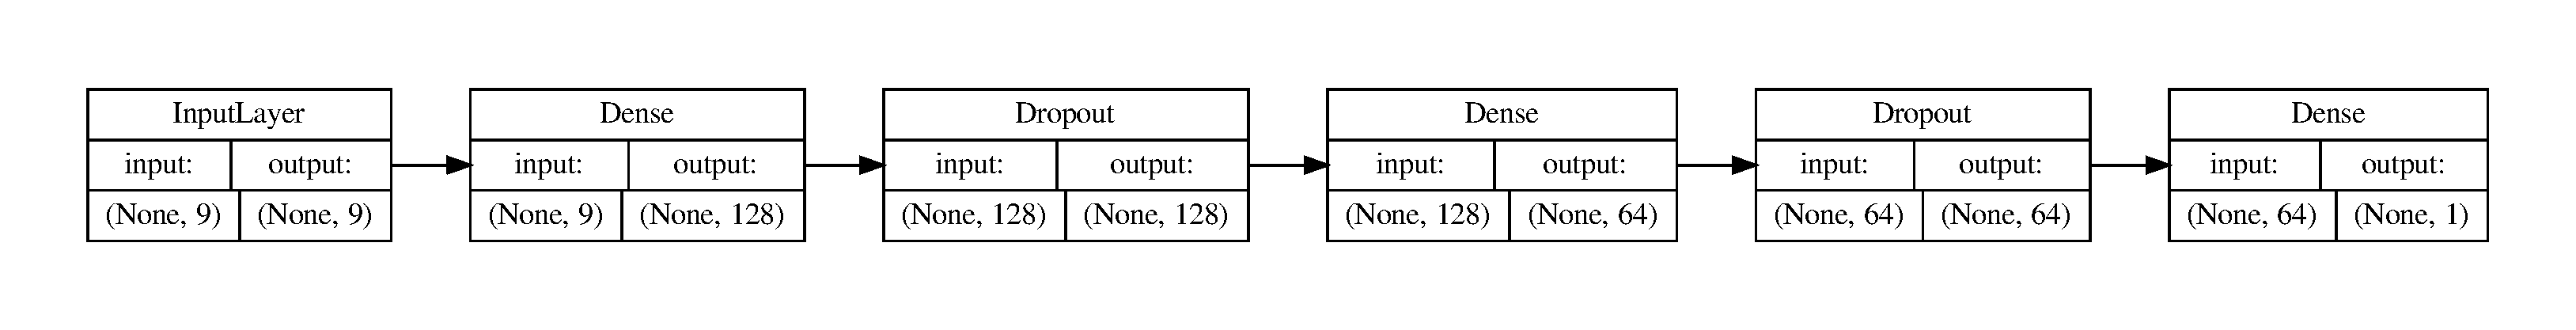
\includegraphics[width=1.2\textwidth]{figures/part2_model.pdf}}%
    \caption{Neural Network Architecture}
    \label{fig:part2model}
\end{figure}
\noindent
More details of the architecture and training parameters are given in \autoref{tab:part2initialnetworkparam}.

% Please add the following required packages to your document preamble:
% \usepackage[table,xcdraw]{xcolor}
% If you use beamer only pass "xcolor=table" option, i.e. \documentclass[xcolor=table]{beamer}
\begin{table}[]
\begin{tabular}{|l|l|l|l|l|l|}
\hline
\rowcolor[HTML]{EFEFEF} 
\textbf{Training Epochs} & \textbf{Batch Size} & \textbf{Activation Function} & \textbf{Dropout} & \textbf{Learning Rate} & \textbf{L2 Regularization} \\ \hline
10                  & 64                  & ReLu                         & 0                & 0.01                   & 0                          \\ \hline
\end{tabular}
\caption[Part 2: Initial Network Hyperparameters]{Initial Network Hyperparameters}
\label{tab:part2initialnetworkparam}
\end{table}
\noindent Owing to the complexity of the dataset, we used relatively large layer sizes in order to capture any interesting interactions between features and the target. The initial model did not significantly overfit the data, and achieved a relatively high (compared to more sophisticated models) AUC-ROC of 0.60. However, this was improved after doing a hyperparameter search which applied appropriate dropout and regularization values, which increased the AUC-ROC to 0.62. The purpose of regularization is to penalise large weights which has the effect of pushing weights toward zero, hence preventing overfitting and leading to more reliable learning.

\subsection{Architecture Evaluation}
\subsubsection*{Metrics}
The classification accuracy with an imbalanced dataset can be misleading. For instance, with the dataset analysed, a classifier predicting only the majority class will still have an classification accuracy of above 90\%.

To appropriately evaluate the performance, we first compute a confusion matrix where the columns represent predicted labels and rows represent ground truth labels. To account for the imbalances, we normalized the confusion matrix by row, i.e., by class, from which the recall and precision were derived.

 Recall is defined as 
\begin{equation}
\textnormal{Recall}=\frac{\textnormal{True Positive}}{\textnormal{True Positive}+\textnormal{False Negative}},
\end{equation}
capturing how well our model predicts the class compared to the true class of the instances. In particular, recall for the minority class was of particular interest to observe how well those who have made claims were being classified.

Precision is defined as
\begin{equation}
\textnormal{Precision}=\frac{\textnormal{True Positive}}{\textnormal{True Positive}+\textnormal{False Positive}},
\end{equation}
and provides a measure of how likely it is that an instance was from a particular class after the model predicted it was from that class. In particular, the precision for the majority class was of particular interest to observe how many of the minority class were being captured when predicted not to have made a claim.

In addition to the above, another key metric for evaluation was the AUC-ROC curve. The receiver operating characteristic (ROC) curve is a plot of the true positive rate against the false positive rate, defined as:
\begin{equation}
\textnormal{FPR}=\frac{\textnormal{False Positive}}{\textnormal{False Positive}+\textnormal{True Negative}},
\end{equation}
\noindent The true positive rate and false positive rate are traced out for every decision boundary, thereby the ROC curve is invariant to class ratios and the decision boundary. The area under the curve (AUC) is a measure of separability between the the classes and represents how well the model is able to distinguish between the the classes. A model with AUC equal to one is able to perfectly distinguish the classes whereas an AUC of 0.5 implies that the model is unable to separate the classes.

\subsubsection*{Initial Performance}

Due to the difficulty of classifying the provided dataset, as elucidated in Section 2.1.1, we strived to obtain a good initial architecture for the model that would be able to capture most of the inherent correlations between features and the target. The results we obtained were are provided in \autoref{tab:res1}.

% Please add the following required packages to your document preamble:
% \usepackage[table,xcdraw]{xcolor}
% If you use beamer only pass "xcolor=table" option, i.e. \documentclass[xcolor=table]{beamer}
\begin{table}[H]
\begin{tabular}{|
>{\columncolor[HTML]{EFEFEF}}l |lll|}
\hline
\textbf{}         & \multicolumn{1}{r|}{\cellcolor[HTML]{EFEFEF}\textbf{Normalized Precision}} & \multicolumn{1}{r|}{\cellcolor[HTML]{EFEFEF}\textbf{Normalized Recall}} & \cellcolor[HTML]{EFEFEF}\textbf{F1-Score} \\ \hline
\textbf{Class 0}  & \multicolumn{1}{r|}{0.59}                                                  & \multicolumn{1}{r|}{0.58}                                               & 0.58                                      \\ \hline
\textbf{Class 1}  & \multicolumn{1}{r|}{0.59}                                                  & \multicolumn{1}{r|}{0.60}                                               & 0.54                                      \\ \hline
\end{tabular}
\hfill
\begin{tabular}{|>{\columncolor[HTML]{EFEFEF}}l|r|}
\hline
\textbf{Accuracy} &  0.58 \\ \hline
\textbf{ROC-AUC}  &  0.60 \\ \hline
\end{tabular}
\caption[Part 2: Initial Network Performance]{Performance of the initial model}
\label{tab:res1}
\end{table}

\subsubsection*{Final Model Performance}

After hyperparameter tuning (see \autoref{sec:hyptune}), our final model had an AUC-ROC of 0.62, as shown in \autoref{tab:res2}.

\begin{table}[H]
\begin{tabular}{|
>{\columncolor[HTML]{EFEFEF}}l |lll|}
\hline
\textbf{}         & \multicolumn{1}{r|}{\cellcolor[HTML]{EFEFEF}\textbf{Normalized Precision}} & \multicolumn{1}{r|}{\cellcolor[HTML]{EFEFEF}\textbf{Normalized Recall}} & \cellcolor[HTML]{EFEFEF}\textbf{F1-Score} \\ \hline
\textbf{Class 0}  & \multicolumn{1}{r|}{0.60}                                                  & \multicolumn{1}{r|}{0.49}                                               & 0.58                                      \\ \hline
\textbf{Class 1}  & \multicolumn{1}{r|}{0.57}                                                  & \multicolumn{1}{r|}{0.67}                                               & 0.54                                      \\ \hline
\end{tabular}
\hfill
\begin{tabular}{|>{\columncolor[HTML]{EFEFEF}}l|r|}
\hline
\textbf{Accuracy} &  0.51 \\ \hline
\textbf{AUC-ROC}  &  0.62 \\ \hline
\end{tabular}
\caption[Part 2: Final Network Performance]{Performance of the final model}
\label{tab:res2}
\end{table}
\noindent
This is a marginal increase from the initial value of 0.60, but for difficult to classify real world data, this incremental increase can affect overall profits of the insurance company significantly. The difference in ROC curves can be seen in \autoref{fig:part2roc}. It is interesting to note that the accuracy went down after tuning, however, as mentioned previously, accuracy is not the best metric for evaluating model performance, and AUC-ROC serves as better estimate given the imbalanced nature of the data. \autoref{fig:part2roc} also shows us that optimizing the hyperparameters makes the graph more symmetrical, and increases the area under the curve, which is an indication of better model performance. 
\begin{figure}
    \centering
    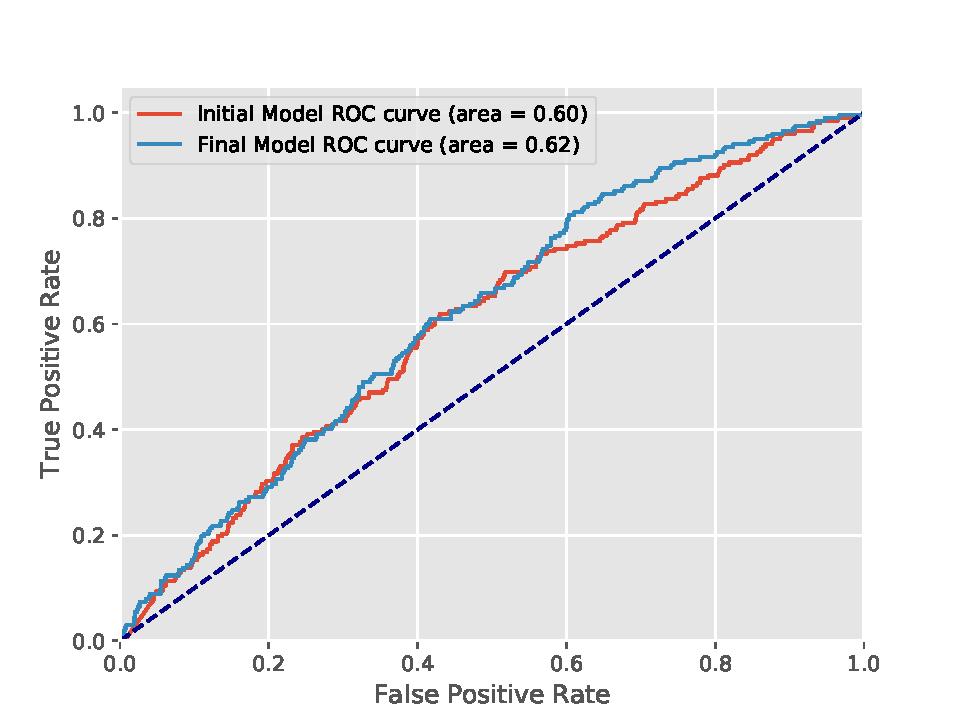
\includegraphics[width=0.7\textwidth]{figures/part2ROC.pdf}
    \caption[Part 2: ROC curves]{Part 2 ROC curves}
    \label{fig:part2roc}
\end{figure}

\subsection{Hyperparameter Tuning}
\label{sec:hyptune}
The key hyperparameters we were looking to optimise were the number of epochs, batch size, activation function, dropout rate, learning rate, and l2 regularization value. We optimised to the AUC-ROC as this provides a gauge of model performance which is independent of the decision boundary. The values used in the search are shown in \autoref{tab:hypparamsearch}.

% Please add the following required packages to your document preamble:
% \usepackage[table,xcdraw]{xcolor}
% If you use beamer only pass "xcolor=table" option, i.e. \documentclass[xcolor=table]{beamer}
\begin{table}[H]
\begin{tabular}{|l|l|l|l|l|l|}
\hline
\rowcolor[HTML]{EFEFEF} 
\textbf{Epoch Size} & \textbf{Batch Size} & \textbf{Activation Function} & \textbf{Dropout} & \textbf{Learning Rate} & \textbf{L2 Regularization} \\ \hline
5                   & 32                  & ReLu                         & 0                & 0.01                   & 0                          \\ \hline
10                  & 64                  & linear                       & 0.1              & 0.001                  & 0.01                       \\ \hline
20                  & 128                 &                              & 0.2              &                        & 0.001                      \\ \hline
                    &                     &                              & 0.3              &                        &                            \\ \hline
\end{tabular}
\caption{Configurations of hyperparameters used in the hyperparameter search.}
\label{tab:hypparamsearch}
\end{table}

The hyperparameter search was done over a search space comprising all combinations of the values shown in \autoref{tab:hypparamsearch}. This resulted in a search space of 432 distinct combinations. The search was done on all combinations at once as optimizing one or two at a time may be faster, but might result in overlooking possible
beneficial interactions between hyperparameter values. Therefore, searching all combinations is the most thorough approach, and is fast when using a GPU. 

\noindent
To carry out the hyperparameter search, we first created a test set comprising 20\% of the data, which was set aside for the final evaluation, with the remaining 80\% used for training and validation. Additionally, the same random seed was used for the initial splitting of the data in every run. This was done to ensure that any changes to model performance were only caused by changes to the hyperparameters, allowing us to reliably explore their effects on the model. We then performed a 5-fold cross-validation on each combination of the the hyperparameters for evaluation purposes. When performing cross-validation, we ensured that oversampling was applied after splitting into training and validation datasets to prevent the synthetically generated samples from also being present in the validation set. This ensured that the validation set only captured trends truly present in the data. Just like the initial model, SMOTE and the removal of Tomek Links (see Data Preprocessing in section 2.1) were used to oversample the datasets. 

The model was then built, compiled and fit to the cross validation datasets, and the average AUC-ROC for all cross validation runs was obtained. AUC-ROC was used as a metric for optimization since the test dataset is unbalanced. Therefore the magnitude of the accuracy measure is influenced highly by the modal class. AUC-ROC however, gives a much better indication of performance between both classes in the unbalanced test set. After the hyperparameter search function has looped over every possible combination of parameters, it returns the combination which achieved the maximum AUC-ROC.

The search process returned the optimal parameters shown in \autoref{tab:fuckmesideways}, which were implemented in the final model.


\begin{table}[H]
\begin{tabular}{|l|l|l|l|l|l|}
\hline
\rowcolor[HTML]{EFEFEF} 
\textbf{Epoch Size} & \textbf{Batch Size} & \textbf{Activation Function} & \textbf{Dropout} & \textbf{Learning Rate} & \textbf{L2 Regularization} \\ \hline
20                  & 32                  & ReLu                         & 0.1              & 0.001                  & 0.01                       \\ \hline
\end{tabular}
\caption[Result of Hyperparameter Search]{Optimal parameters found from hyperparameter search}
\label{tab:fuckmesideways}
\end{table}










